I principali effetti del worm Code Red furono il degradamento delle prestazioni e la perdità di stabilità dei sistemi coinvolti. Il costo globale complessivo stimato fu di 2.6 miliardi di dollari \cite{ce, sans}, di cui 1.1 miliardi impiegati nell’ispezione ed il recupero dei server ed i restanti 1.5 miliardi riguardarono le perdite di produttività a seguito dell’indisponibilità dei sistemi.\\
Quest’ultimi comprendevano non soltanto le macchine server degli utenti finali, ma anche vaste porzioni dell’infrastruttura di rete che furono completamente disabilitate, molte compagnie provider di dispositivi di rete sperimentarono un’indisponibiltà media di ben 36 ore \cite{sans}.\\
Il processo di propagazione del worm ha generato un’enorme quantità di pacchetti. Sebbene il volume di questi pacchetti era relativamente piccolo rispetto al normale traffico di rete, l’ingente quantità ha causato congestionamento e gravi problemi ad alcuni ruoter, specialmente quelli con risorse limitate. Per esempio, a causa della generazione randomica degli indirizzi IP, molti pacchetti non venivano inoltrati poiché la destinazione risultava sconosciuta, finendo così per riempire le cache ARP, esaurire la memoria e provocare il riavvio dei dispositivi \cite{cisco}.\\
La figura ~\ref{impatto} mostra il costo complessivo di Code Red in relazione agli incidenti più rilevanti del periodo \cite{ce}.

\begin{figure}[!hbp]
\centering
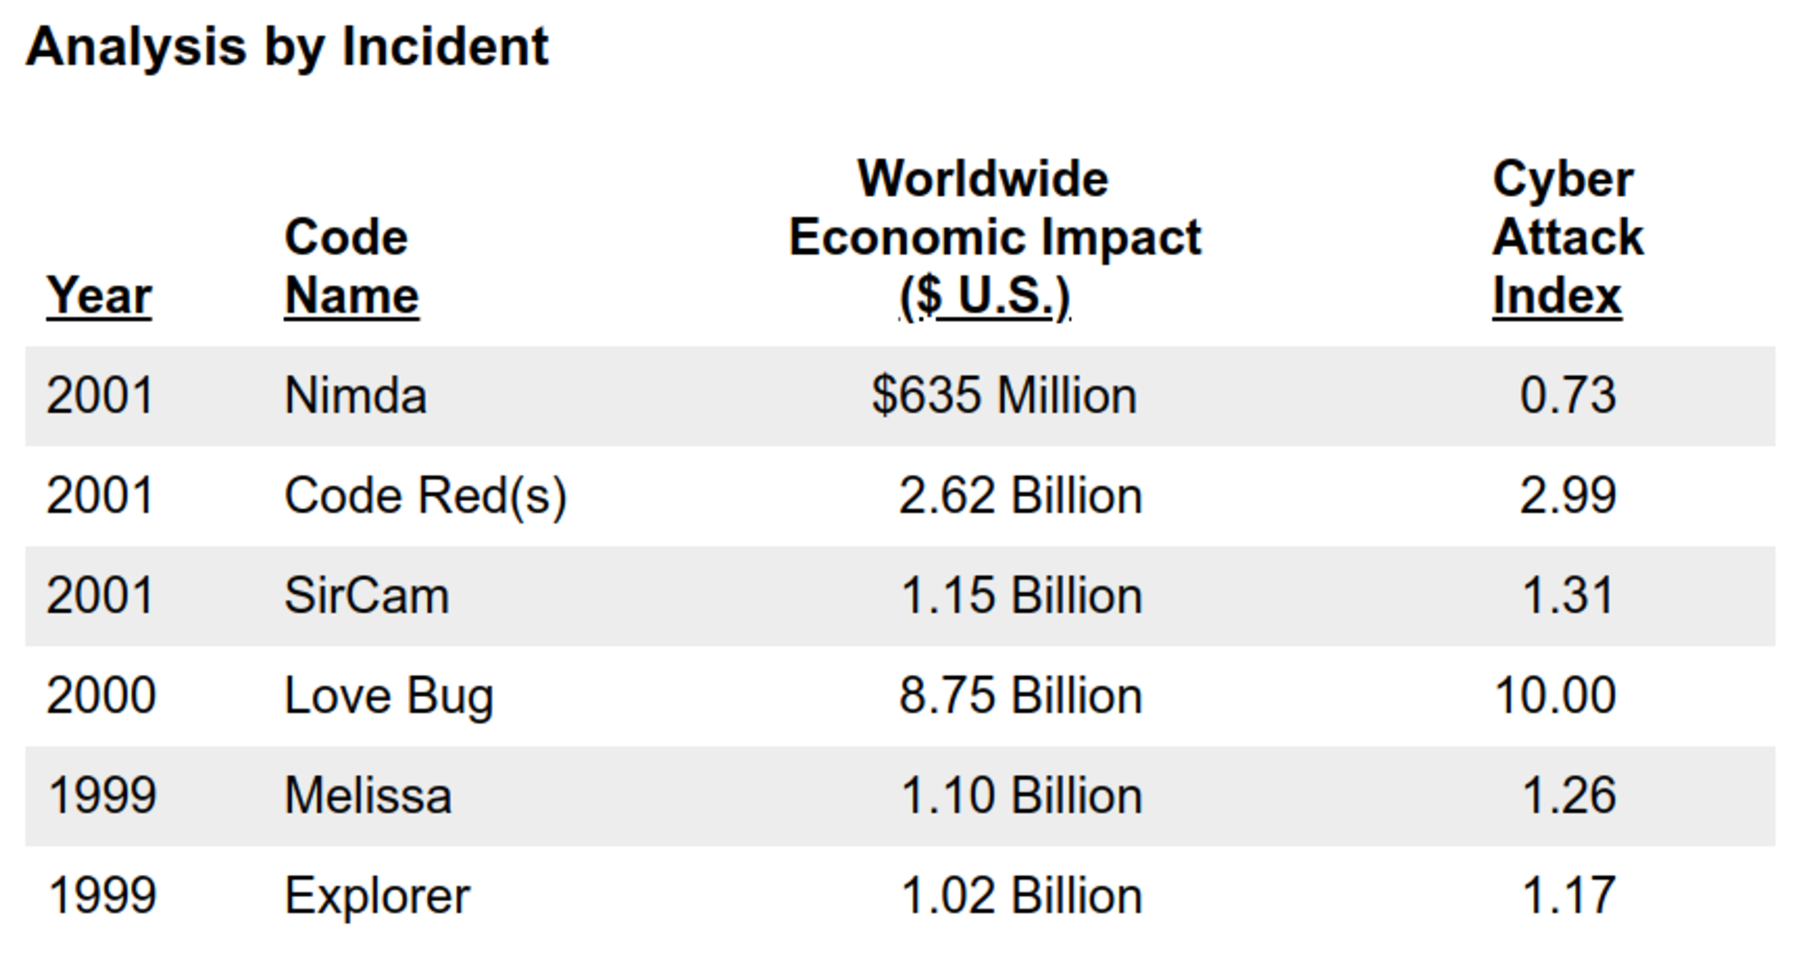
\includegraphics[width=0.5\textwidth]{images/impatto.eps}
\caption{confronto danno economico}
\label{impatto}
\end{figure}

Il sito web della Casa Bianca riuscì ad evitare conseguenze sostanzialmente “disattivando” l’indirizzo IP bersaglio dell’attacco DDoS, ovvero reindirizzando tutte le richieste non malevole verso altri indirizzi associati, questo è stato possibile perché il worm è stato progettato per inviare traffico verso un unico indirizzo IP, invece dell’intero blocco di indirizzi relativi al dominio della Casa Bianca.

